\subsection{Подход Клайнберга}

Следующий подход предложил Американский математик Джон Клайнберг. Перед началом разбора,
мне бы хотелось сделать некоторую поправку. Джон Клайнберг в своих статьях нигде не 
упоминает о коэффиценте класстеризации. Вместо этого он говорит только о наличии длинных
и коротких рёбер. Это немного расширяет класс "Тесных" графов, однако идейно 
ничего не меняет.

    Изучим заново граф, который изображён на Рис. \ref{lattice}. Он состоит только из
коротких связей, а значит, тесным графом не является. Есть разные способы решить эту проблему,
давайте рассмотрим предложение Джона Клайнберга, так как его метод формирования длинных
рёбер очень естественно вписывается в окружающий нас мир. Идея проста: чем человек дальше от меня, тем меньше
вероятность нашего знакомства. Формально это можно записать так:

\begin{equation} \label{edges_distribution}
    P(u \rightarrow v) = \frac{1}{d(u, v)^r}\frac{1}{C}, \text{ где } C = \sum_{u \neq z \in V}\frac{1}{d(u, z)^r}
\end{equation}

Во время своего исследования, он пришёл к выводу, что наилучший результат достигается при 
r = d, где d - размерность пространства. Причём кол-во длинных рёбер должно быть 
примерно равно $q = \log{n}$. Так как: TODO:

Воспользуемся данной техникой для построения графа в общем случае: Для построения структуры 
по методу Клайнберго необходимо для каждой вершины v пройтись по всему графу, выбрать ближайших
соседей, связать их с v и посчитать константу $C = \sum_{v \neq z \in V}\frac{1}{d(v, z)^r}$ на будущее.
После завершения, останется только выбрать $q = \log{n}$ длинных связей, опираясь на распределение выше 
(\ref{edges_distribution}), и связать их с v.

Однако хочу заметить, что данный алгоритм можно немного упростить, если заметить, что в
построение коротких рёбер здесь нет необходимости. Обосновать это очень просто, близкие связи
будут образовываться сами собой, так как вероятность появления коротких рёбер будет значительно выше, 
чем длинных. Блок схема алгоритма изображена на рис. \ref{Kleinberg_graph_block_scheme}, 

\begin{figure}[H]
    \centering
    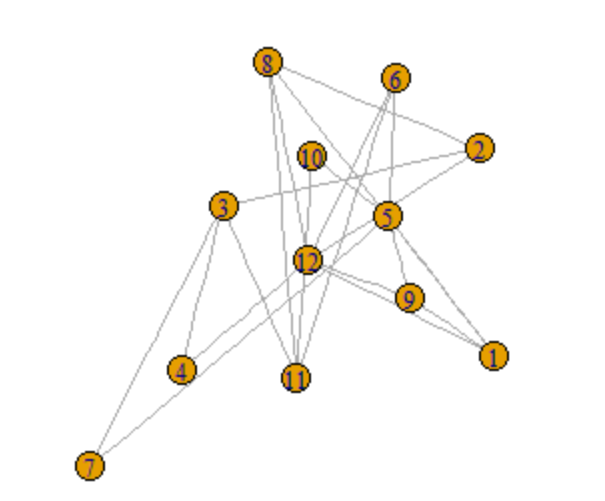
\includegraphics[scale=0.3]{./pictures/random_graph.png}
    \caption{Блок схема построение графа по методу Джона Клайнберга} \label{Kleinberg_graph_block_scheme}
\end{figure}

